\documentclass{sintefbeamer}

% packages, font, color, and newcommands
\usepackage{amsfonts, amsmath, oldgerm, lmodern, bm}
\usepackage[font={footnotesize}]{caption}

\usefonttheme{serif}
% \themecolor{blue} 
% meta-data
\title{A phenomenological description of pairwise interactions in emulsion.}
\subtitle{Based on the nearest particle statistic.}
\author{\href{http://basilisk.fr/sandbox/fintzin/Rising-Suspenion/RS.c}{\underline{Fintzi Nicolas}, JL Pireson and S Popinet. }}
\date{Created on May 22, 2022}

\titlebackground{image/pic/bulles.png}

% document body
\begin{document}
\maketitle
\section*{Context}

\begin{frame}{How to accurately predict to coalesce of a pair of droplets ?}

\begin{enumerate}
  \item Needs :
  \begin{itemize}
    \item Model poly disperse emulsion with Population Balance Models. 
    \item Accurate closure terms for the source term of coalesce. 
    \item Accurate prediction of 
    % \item But coalescence models are defined for restricted type of interactions. 
    % \item So which model is the most accurate for modeling coalescence in emulsions ?
  \end{itemize}
  \item Objective :
  \begin{itemize}
    \item Identifying the average relative interactions between the pairs of drops colliding.  
    \item Create statistic of the most representative parameters.
    \item Choose and complete the theoretical models considering the statistical approach.   
  \end{itemize}
\end{enumerate}
\end{frame}

\section*{Theoretical model}
\begin{frame}{How to characterize a collision in a system oil/water ?}
\begin{figure}[h!]
  \centering
  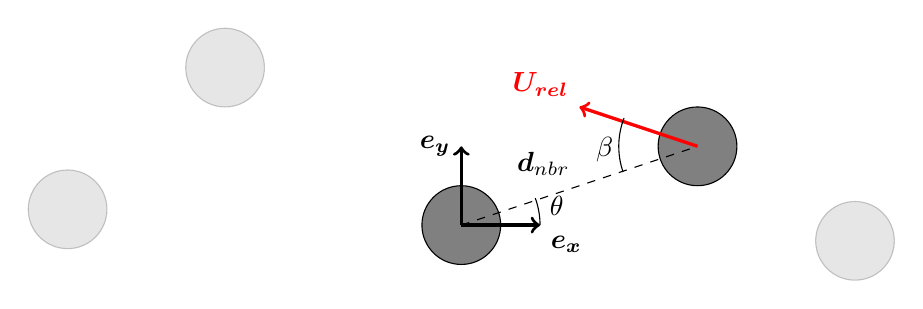
\begin{tikzpicture}
      \draw[fill=gray](0,0)circle (0.5);
      \draw[fill=gray](3,1)circle (0.5);
      \draw[fill=gray,opacity=0.2](5,-0.2)circle (0.5);
      \draw[fill=gray,opacity=0.2](-3,2)circle (0.5);
      \draw[fill=gray,opacity=0.2](-5,0.2)circle (0.5);
      \draw[dashed](0,0)--(3,1)node[midway,above left]{$\bm{d}_{nbr}$};
      \draw[very thick,->,red](3,1)--++(-1.5,0.5)node[above left]{$\bm{U_{rel}}$};
      \draw[very thick,->](0,0)--++(1,0)node[below right]{$\bm{e_x}$};
      \draw[very thick,->](0,0)--++(0,1)node[left]{$\bm{e_y}$};
      \draw(3,1)++(199:1)node[above left]{$\beta$} arc(199:159:1);
      \draw(0,0)++(0:1)node[above right]{$\theta$} arc(0:20:1);
  \end{tikzpicture} 
  \caption{Scheme of a droplet indexed $\alpha =1$ and its nearest neighbor, $\alpha = 2$. The velocity is considered in the frame of the first drop thus, $\bm{U}_{rel} =  \bm{u}_2-\bm{u}_1$ with $\bm{u}_1$ and $\bm{u}_2$ the velocities of the first and second drop. The distance between the two drop, $\bm{d}_{nbr} = \bm{y}_2 -\bm{y}_1$, and its norm $d_{nbr} = |\bm{d}_{nbr}|$. }
\end{figure}
$\triangleright$ We define, $P(\theta,\beta,d_{nbr},u_{rel},t)$, as the probability of finding a pair of particles being in the configuration $\theta,\beta,d_{nbr},u_{rel}$ at time $t$.
\end{frame}
\begin{frame}{How to characterize a collision in a system oil/water ?}
\begin{figure}[h!]
  \centering
  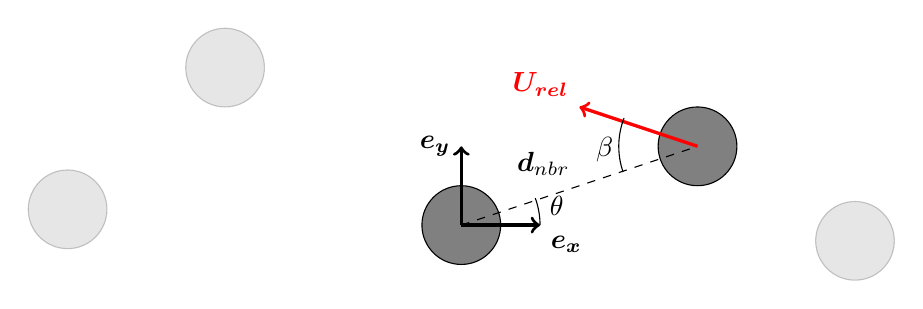
\begin{tikzpicture}
      \draw[fill=gray](0,0)circle (0.5);
      \draw[fill=gray](3,1)circle (0.5);
      \draw[fill=gray,opacity=0.2](5,-0.2)circle (0.5);
      \draw[fill=gray,opacity=0.2](-3,2)circle (0.5);
      \draw[fill=gray,opacity=0.2](-5,0.2)circle (0.5);
      \draw[dashed](0,0)--(3,1)node[midway,above left]{$\bm{d}_{nbr}$};
      \draw[very thick,->,red](3,1)--++(-1.5,0.5)node[above left]{$\bm{U_{rel}}$};
      \draw[very thick,->](0,0)--++(1,0)node[below right]{$\bm{e_x}$};
      \draw[very thick,->](0,0)--++(0,1)node[left]{$\bm{e_y}$};
      \draw(3,1)++(199:1)node[above left]{$\beta$} arc(199:159:1);
      \draw(0,0)++(0:1)node[above right]{$\theta$} arc(0:20:1);
  \end{tikzpicture} 
  \caption{Scheme of a droplet indexed $\alpha =1$ and its nearest neighbor, $\alpha = 2$. The velocity is considered in the frame of the first drop thus, $\bm{U}_{rel} =  \bm{u}_2-\bm{u}_1$ with $\bm{u}_1$ and $\bm{u}_2$ the velocities of the first and second drop. The distance between the two drop, $\bm{d}_{nbr} = \bm{y}_2 -\bm{y}_1$, and its norm $d_{nbr} = |\bm{d}_{nbr}|$. }
\end{figure}
$\triangleright$  It is possible to define subgroups of $P(\theta,\beta,d_{nbr},u_{rel})$ by integrating over the other variables :

$P_{d_{ndr}}(d_{ndr}) = \iint P(\bm{\lambda}) du_{rel}d\theta d\beta.$\hfill
 $P_{\beta\theta}(\beta,\theta) = \iint P(\bm{\lambda}) du_{rel} dd_{ndr}.$
\end{frame}
\section*{results}
\begin{frame}{Radial distribution function of the nearest particle}
  \begin{figure}[h!]
    \centering
    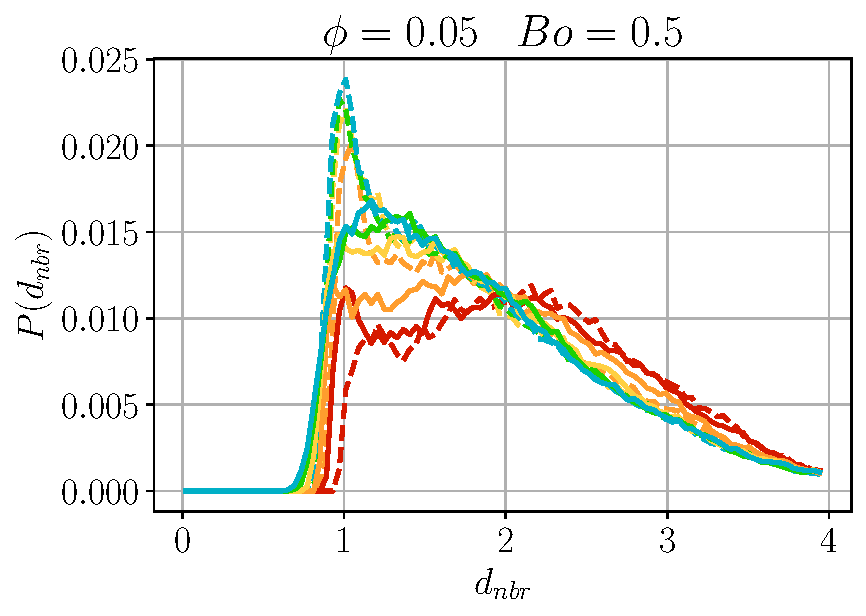
\includegraphics[width=0.33\textwidth]{image/N_10/Pcond/probaNBo0_5PHI0_05.pdf}
    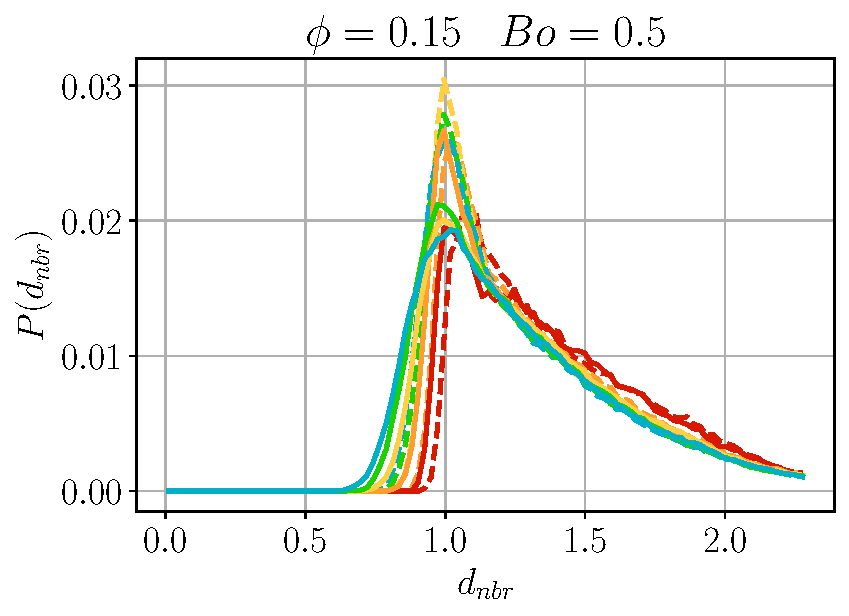
\includegraphics[width=0.33\textwidth]{image/N_10/Pcond/probaNBo0_5PHI0_15.pdf}
    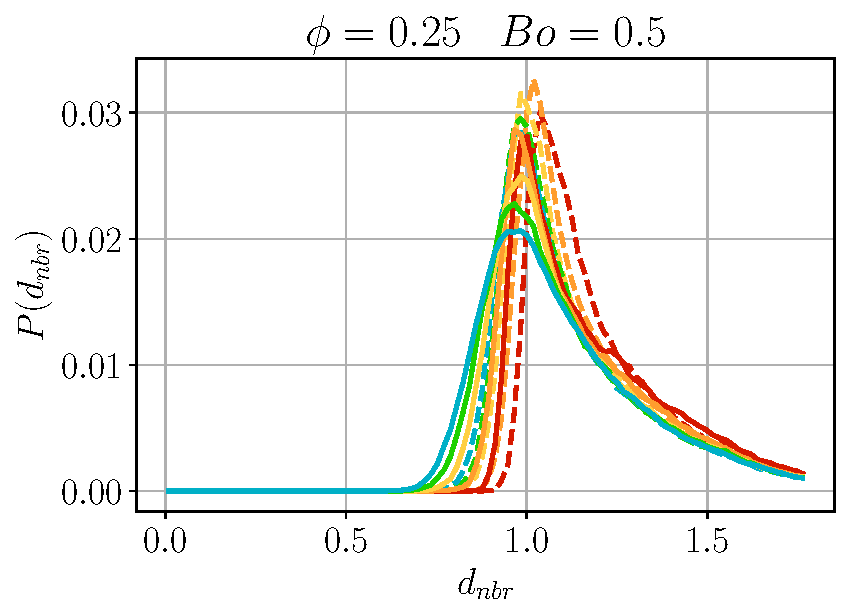
\includegraphics[width=0.33\textwidth]{image/N_10/Pcond/probaNBo0_5PHI0_25.pdf}
    % 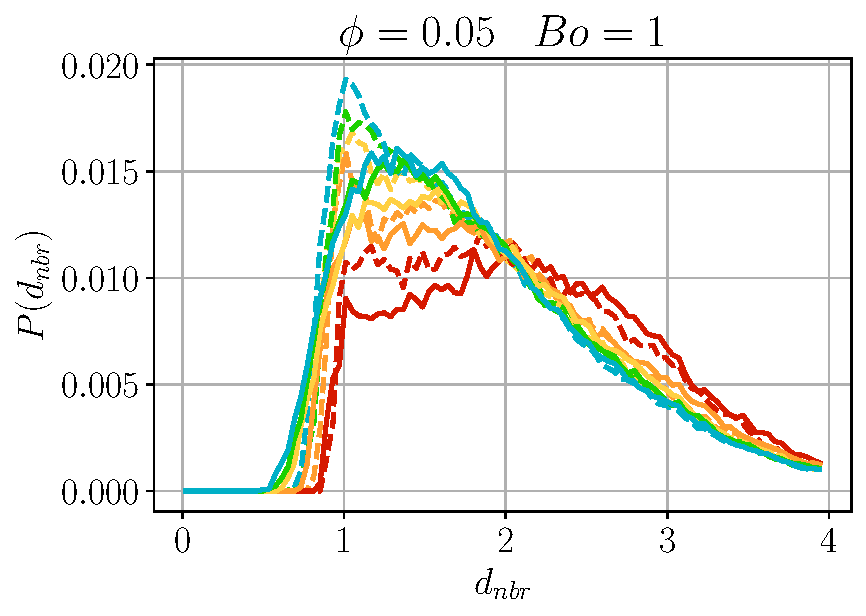
\includegraphics[width=0.33\textheight]{image/N_10/Pcond/probaNBo1PHI0_05.pdf}
    % 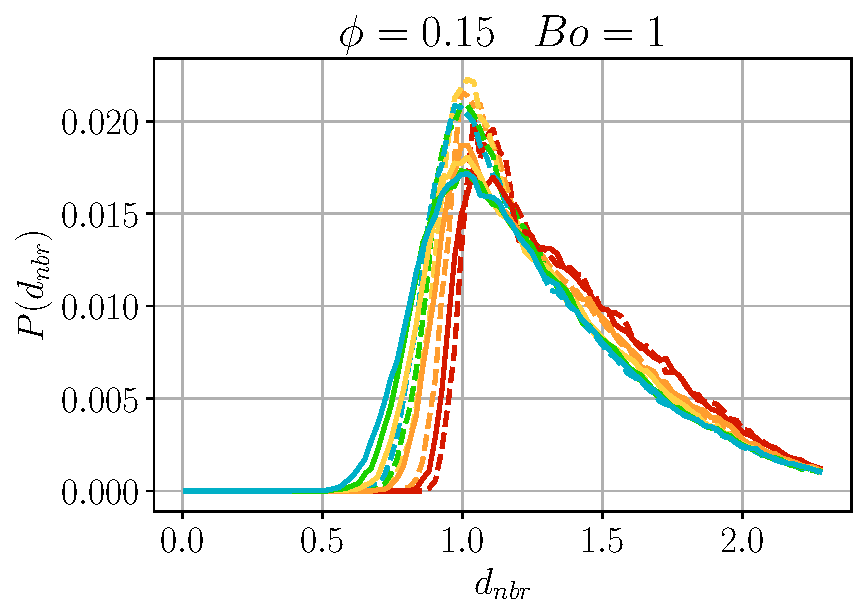
\includegraphics[width=0.33\textheight]{image/N_10/Pcond/probaNBo1PHI0_15.pdf}
    % 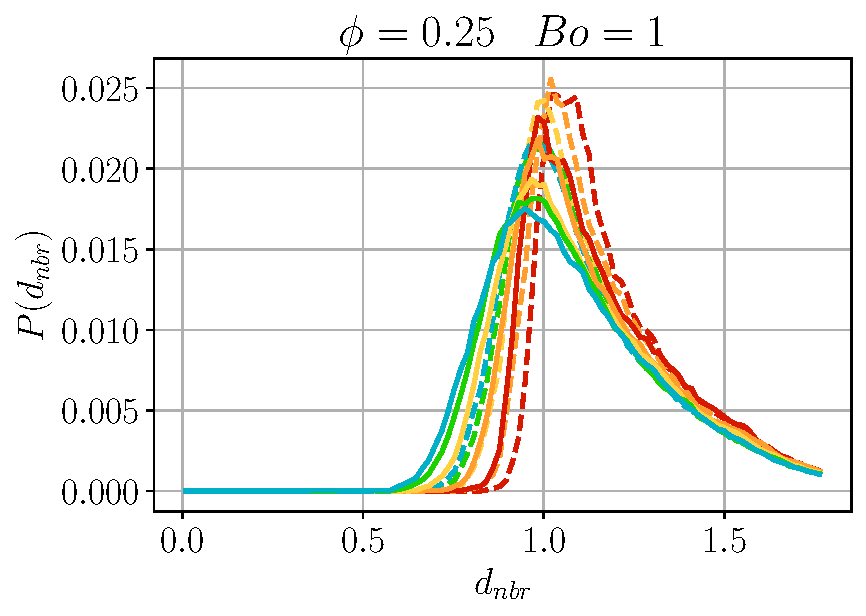
\includegraphics[width=0.33\textheight]{image/N_10/Pcond/probaNBo1PHI0_25.pdf}
    \caption{Probability density function in terms of the nearest particle distance $|\bm{d}_{nbr}|$. Dashed lines : $\mu_f = 0.042$, solid lines : $\mu_f = 0.42$. $Ga = [10; 100]$ from red to blue. }  
    \label{fig:Pdmin}
\end{figure}
\begin{itemize}
  \item Viscosity ratio : $\mu_r = \mu_d / \mu_f$ 
  \item $Bo$ is the \textit{Bond} number.  
  \item $\phi$ is the volume fraction of droplets.  
\end{itemize}
\end{frame}

\begin{frame}{Radial distribution function of the nearest particle}
  \begin{figure}[h!]
    \centering
    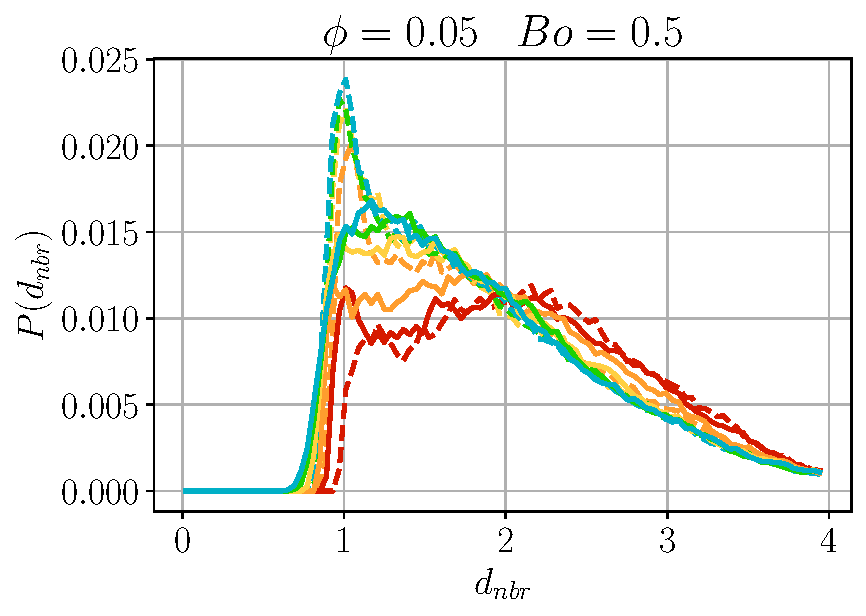
\includegraphics[width=0.33\textwidth]{image/N_10/Pcond/probaNBo0_5PHI0_05.pdf}
    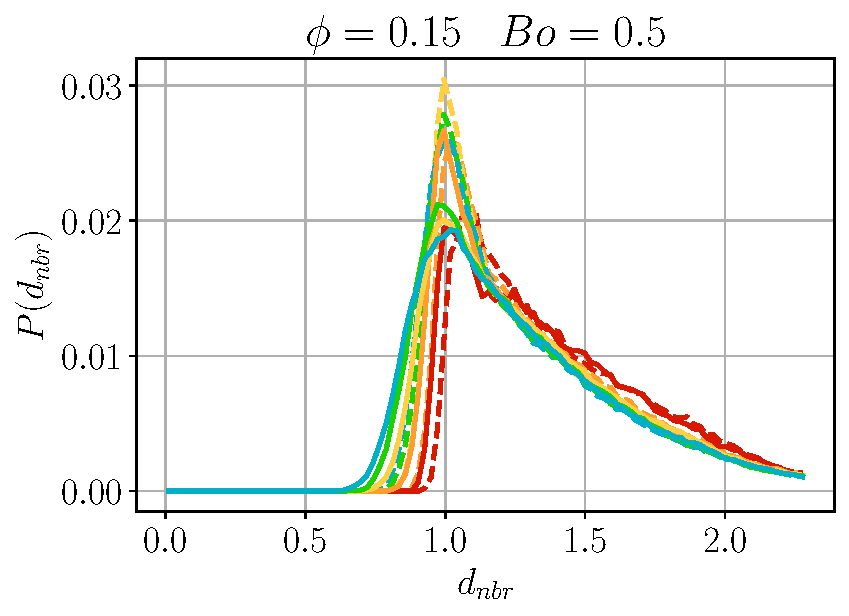
\includegraphics[width=0.33\textwidth]{image/N_10/Pcond/probaNBo0_5PHI0_15.pdf}
    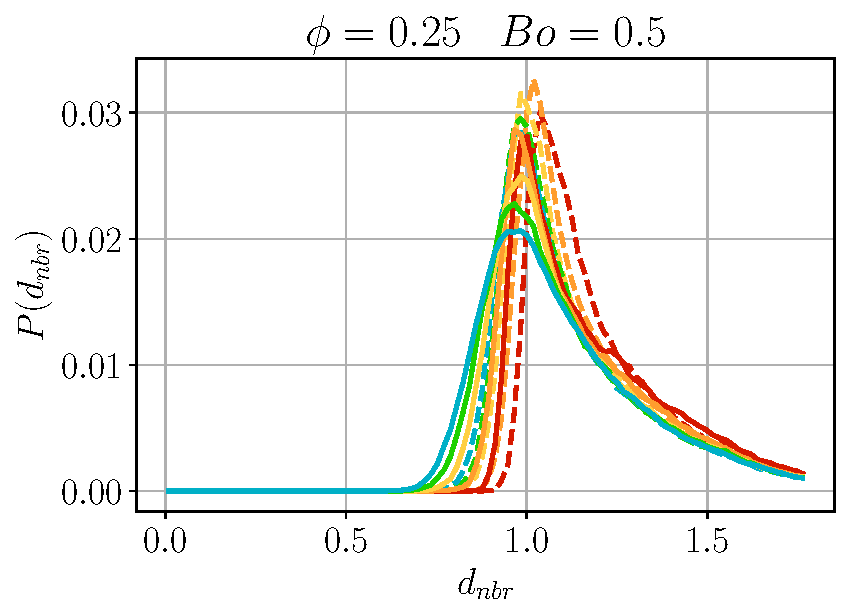
\includegraphics[width=0.33\textwidth]{image/N_10/Pcond/probaNBo0_5PHI0_25.pdf}
    % 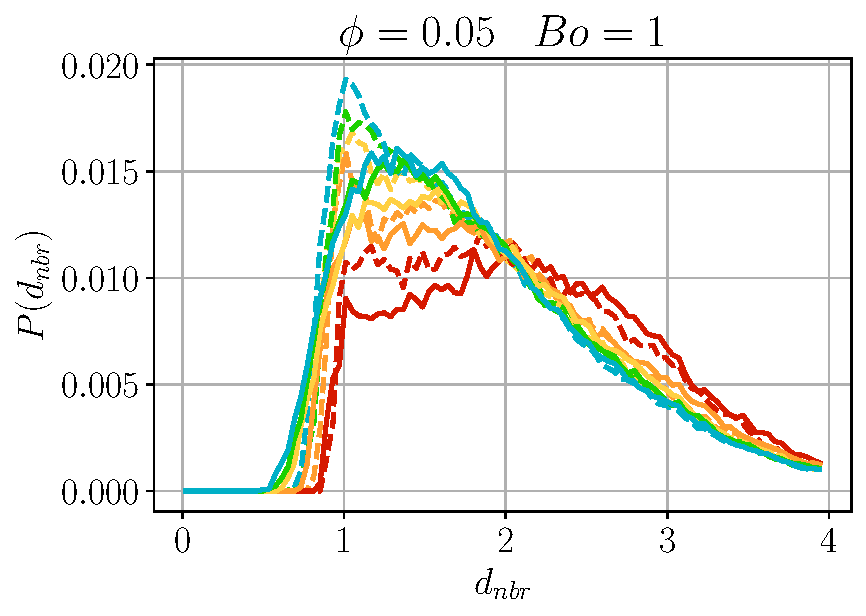
\includegraphics[width=0.33\textheight]{image/N_10/Pcond/probaNBo1PHI0_05.pdf}
    % 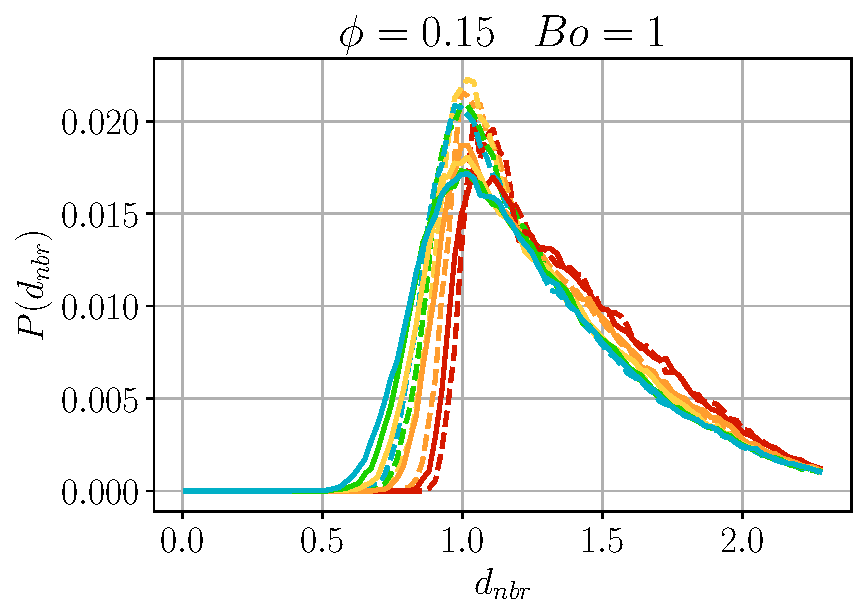
\includegraphics[width=0.33\textheight]{image/N_10/Pcond/probaNBo1PHI0_15.pdf}
    % 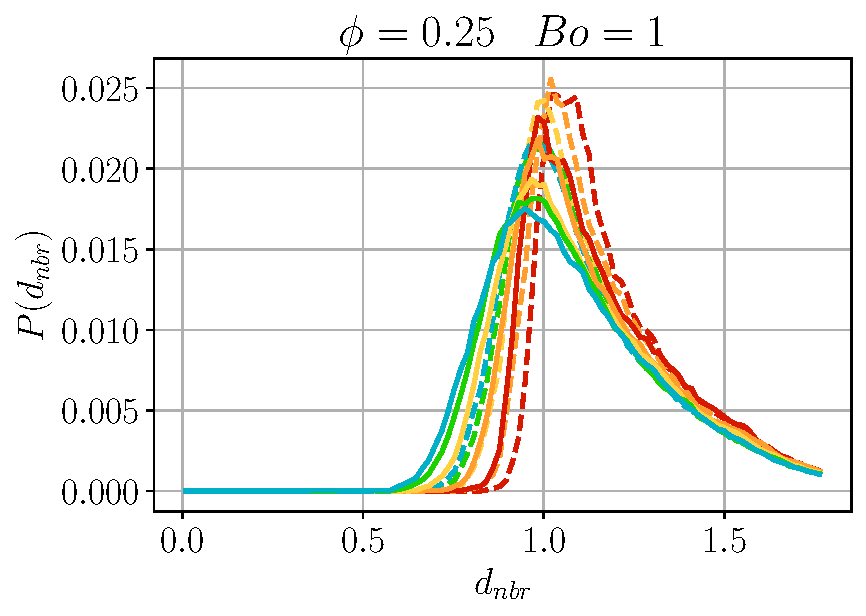
\includegraphics[width=0.33\textheight]{image/N_10/Pcond/probaNBo1PHI0_25.pdf}
    \caption{Probability density function in terms of the nearest particle distance $|\bm{d}_{nbr}|$. Dashed lines : $\mu_f = 0.042$, solid lines : $\mu_f = 0.42$. $Ga = [10; 100]$ from red to blue. }  
\end{figure}
$\triangleright$ The particles get closer for increasing $\phi$ and decreasing $\mu_r$.
\end{frame}
\begin{frame}{Radial distribution function of the nearest particle}
  \begin{figure}[h!]
    \centering
    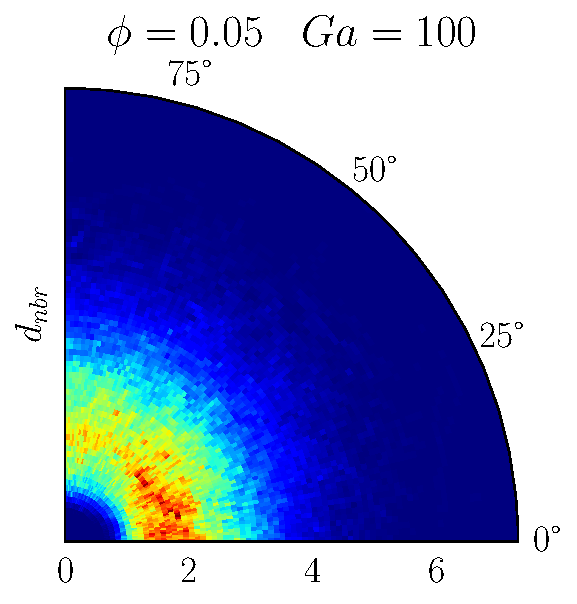
\includegraphics[width =0.3\textwidth]{image/N_10/beta/2DMAP_theta_distmin_dmin_10_Bo1PHI0_05mu_r0_42Ga100.pdf}
    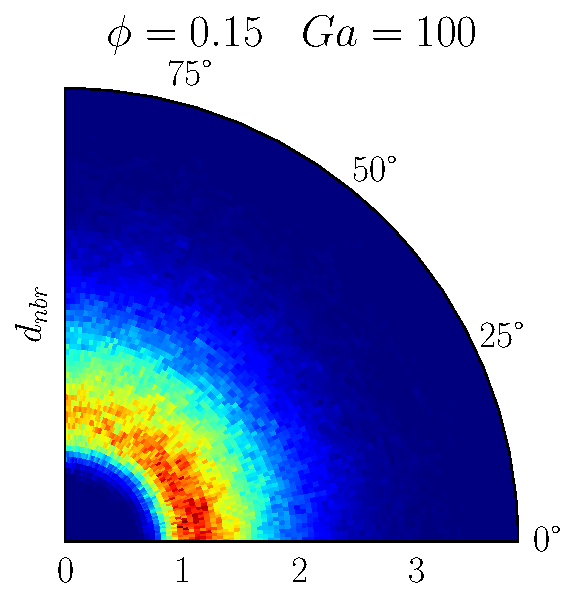
\includegraphics[width =0.3\textwidth]{image/N_10/beta/2DMAP_theta_distmin_dmin_10_Bo1PHI0_15mu_r0_42Ga100.pdf}
    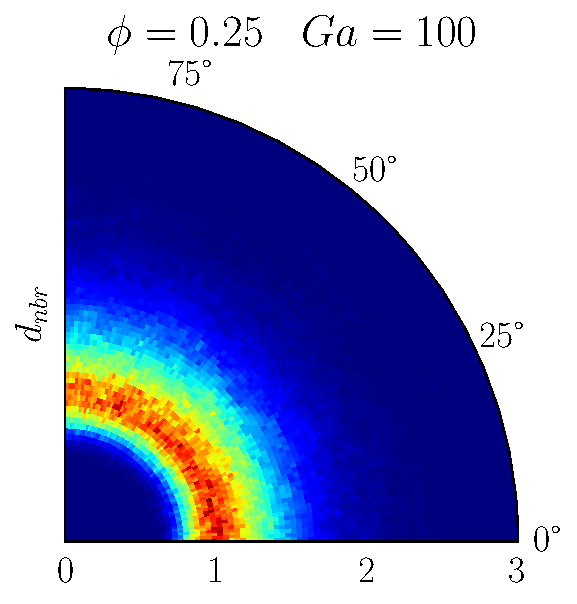
\includegraphics[width =0.3\textwidth]{image/N_10/beta/2DMAP_theta_distmin_dmin_10_Bo1PHI0_25mu_r0_42Ga100.pdf}
    \caption{2 plots of $P_{d_{nbr}\theta}(d_{nbr},\theta)$ for different $\phi$ and $Ga$ at $Bo = 1$ and $\mu_r = 0.42$. The color represents the density, it goes from blue meaning $P_{d_{nbr}\theta}(d_{nbr},\theta)= P_{min}$, to red meaning $P_{d_{nbr}\theta}(d_{nbr},\theta) = P_{max}$.} 
\end{figure} 
$\triangleright$ The nearest particles arrange horizontally for at low $\phi$.
\end{frame}

\begin{frame}{Radial distribution function of the nearest particle}
  \begin{figure}[h!]
    \centering
    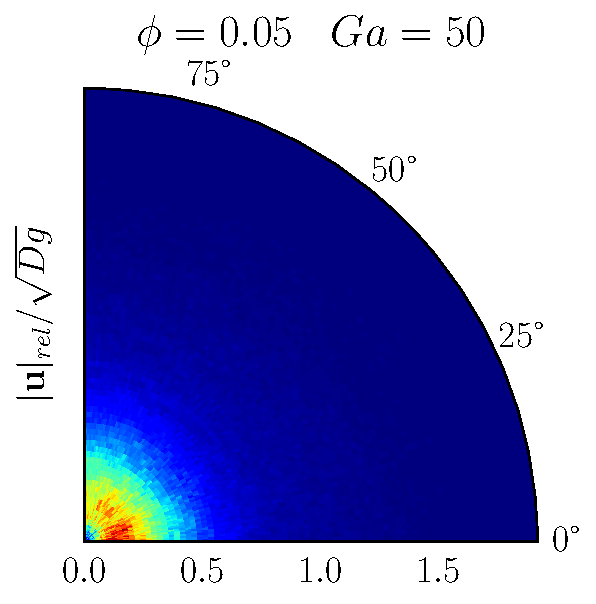
\includegraphics[width =0.3\textwidth]{image/N_10/beta/2DMAP_theta_v_rel_dmin_10_Bo1PHI0_05mu_r0_42Ga50.pdf}
    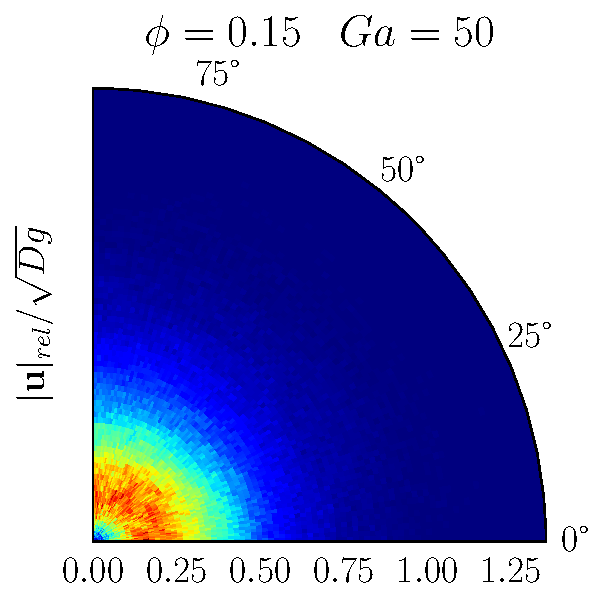
\includegraphics[width =0.3\textwidth]{image/N_10/beta/2DMAP_theta_v_rel_dmin_10_Bo1PHI0_15mu_r0_42Ga50.pdf}
    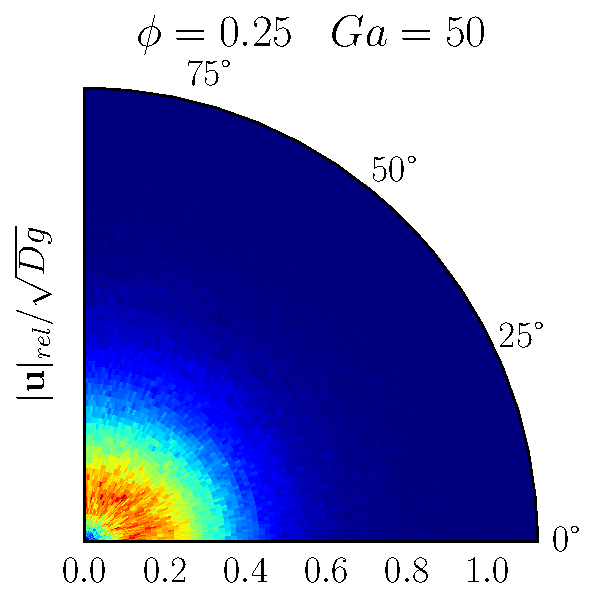
\includegraphics[width =0.3\textwidth]{image/N_10/beta/2DMAP_theta_v_rel_dmin_10_Bo1PHI0_25mu_r0_42Ga50.pdf}
    \caption{2 plots of $P_{|u_{rel}|\theta}(|u_{rel}|,\theta)$ for different $\phi$ and $Ga$ at $Bo = 1$ and $\mu_r = 0.42$. The color represents the density, it goes from blue meaning $P_{|u_{rel}|\theta}(|u_{rel}|,\theta)= 0$, to red meaning $P_{|u_{rel}|\theta}(|u_{rel}|,\theta) = P_{max}$.} 
\end{figure} 
$\triangleright$ Similarly, the relative velocity  becomes independent of $\theta$ at high $\phi$.
\end{frame}


\begin{frame}{2D density function of the angles distribution}  
\begin{figure}[h!]
    \centering
    
    % 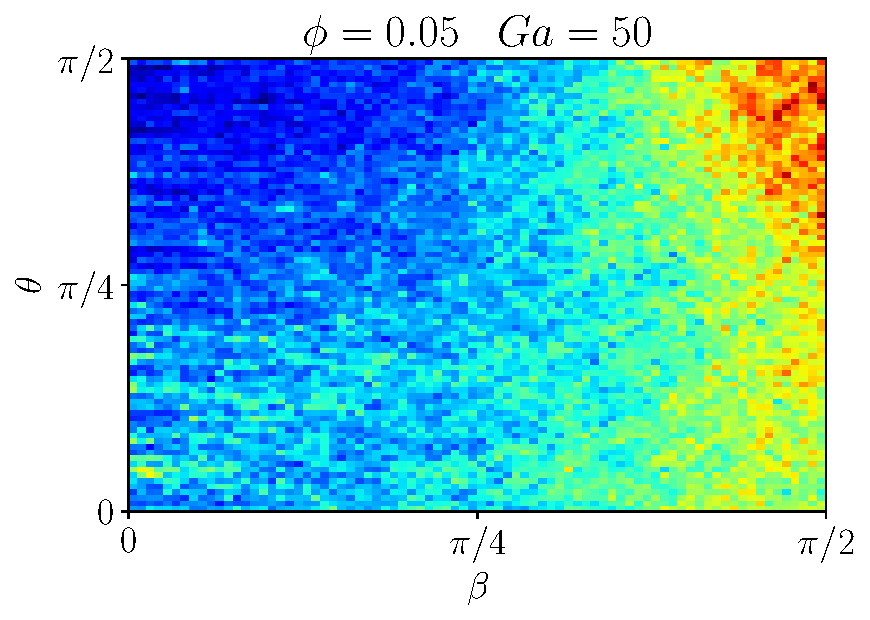
\includegraphics[width = 0.33\textwidth]{image/N_10/beta/2DMAP_beta_theta_dmin_10_Bo0_5PHI0_05mu_r0_042Ga50.pdf}
    % 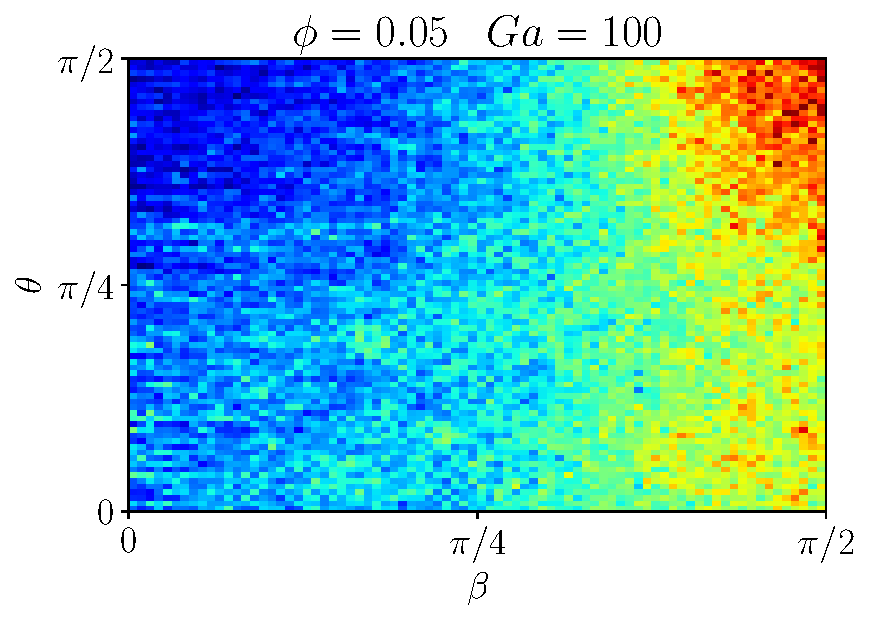
\includegraphics[width = 0.33\textwidth]{image/N_10/beta/2DMAP_beta_theta_dmin_10_Bo0_5PHI0_05mu_r0_042Ga100.pdf}
    % 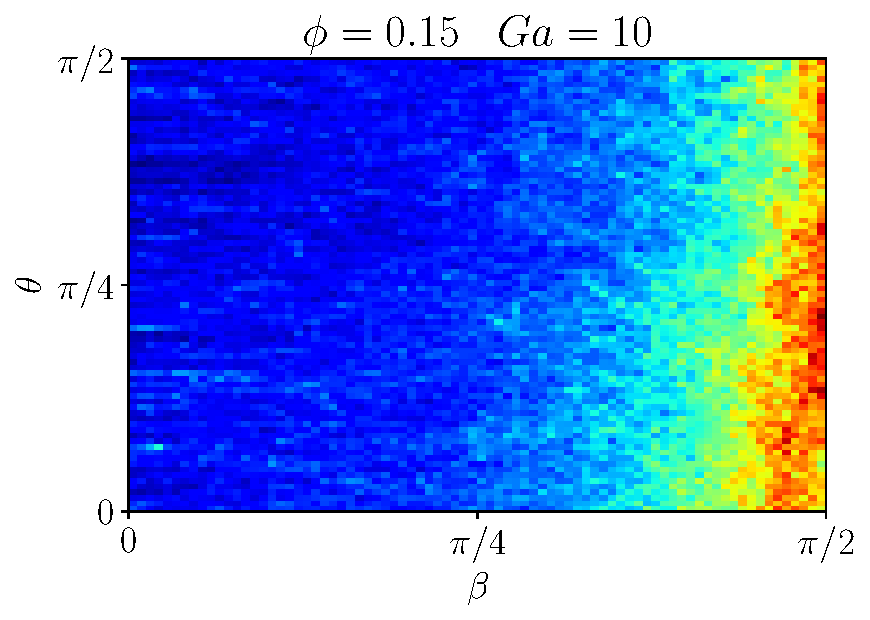
\includegraphics[width = 0.33\textwidth]{image/N_10/beta/2DMAP_beta_theta_dmin_10_Bo0_5PHI0_15mu_r0_042Ga10.pdf}
    % 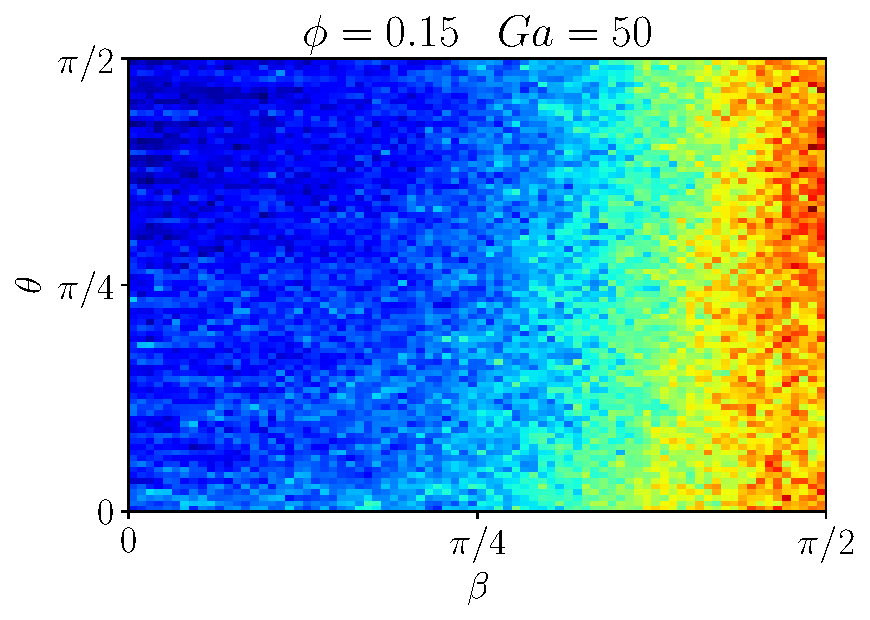
\includegraphics[width = 0.33\textwidth]{image/N_10/beta/2DMAP_beta_theta_dmin_10_Bo0_5PHI0_15mu_r0_042Ga50.pdf}
    % 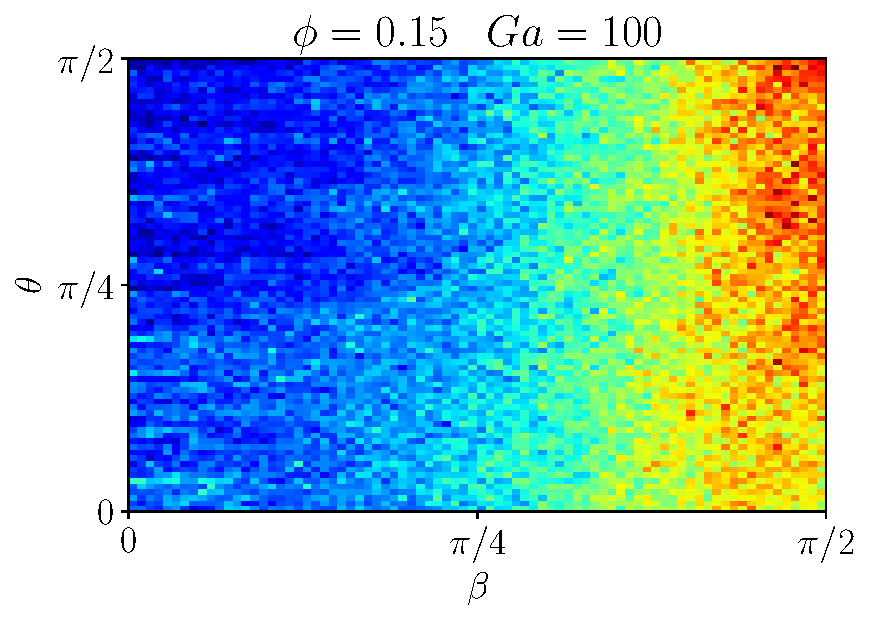
\includegraphics[width = 0.33\textwidth]{image/N_10/beta/2DMAP_beta_theta_dmin_10_Bo0_5PHI0_15mu_r0_042Ga100.pdf}
    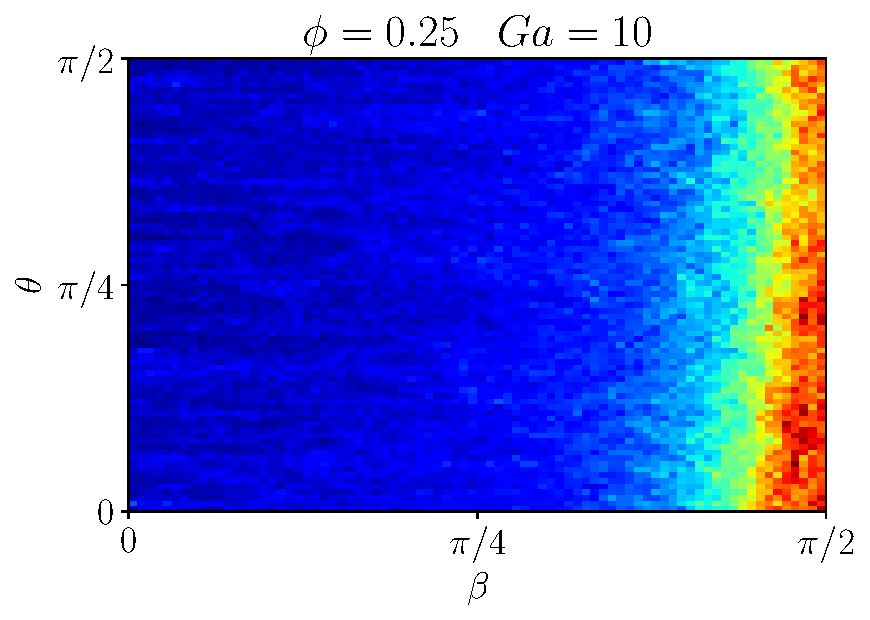
\includegraphics[width = 0.33\textwidth]{image/N_10/beta/2DMAP_beta_theta_dmin_10_Bo0_5PHI0_25mu_r0_042Ga10.pdf}
  %  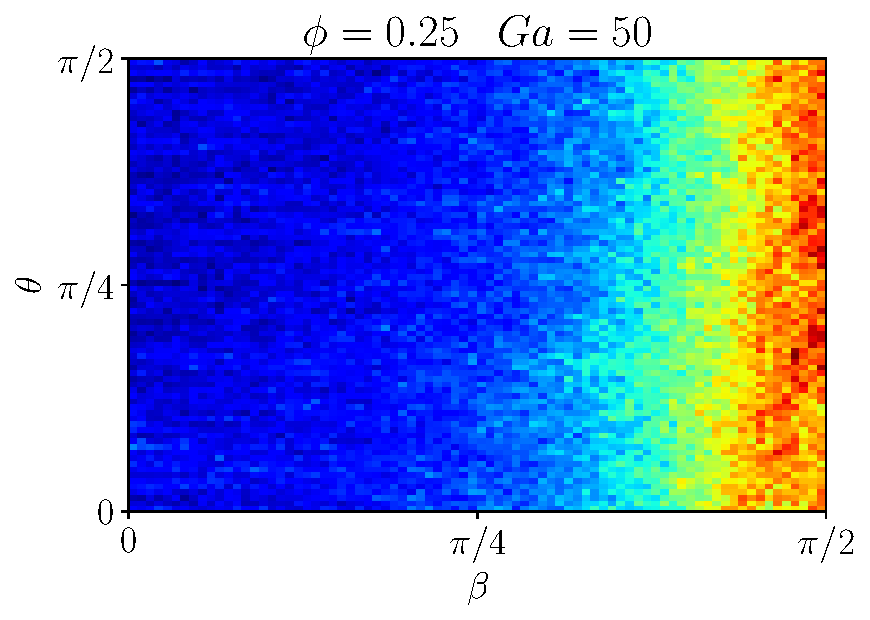
\includegraphics[width = 0.33\textwidth]{image/N_10/beta/2DMAP_beta_theta_dmin_10_Bo0_5PHI0_25mu_r0_042Ga50.pdf}
   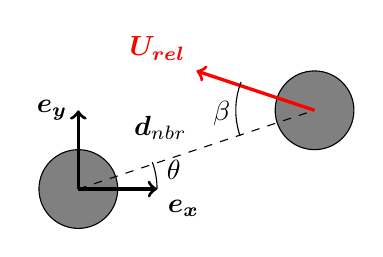
\begin{tikzpicture}
    \draw[fill=gray](0,0)circle (0.5);
    \draw[fill=gray](3,1)circle (0.5);
    \draw[dashed](0,0)--(3,1)node[midway,above left]{$\bm{d}_{nbr}$};
    \draw[very thick,->,red](3,1)--++(-1.5,0.5)node[above left]{$\bm{U_{rel}}$};
    \draw[very thick,->](0,0)--++(1,0)node[below right]{$\bm{e_x}$};
    \draw[very thick,->](0,0)--++(0,1)node[left]{$\bm{e_y}$};
    \draw(3,1)++(199:1)node[above left]{$\beta$} arc(199:159:1);
    \draw(0,0)++(0:1)node[above right]{$\theta$} arc(0:20:1);
  \end{tikzpicture} 
   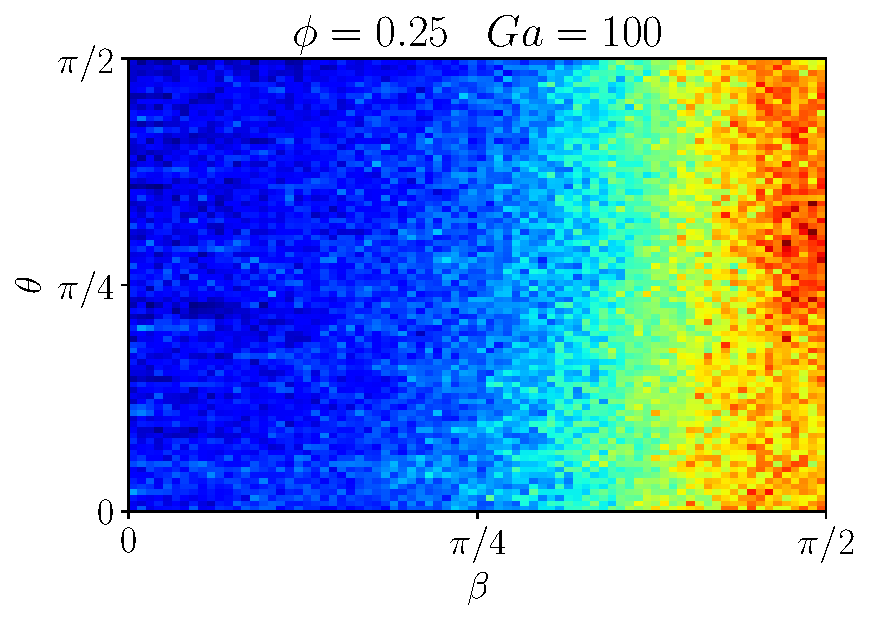
\includegraphics[width = 0.33\textwidth]{image/N_10/beta/2DMAP_beta_theta_dmin_10_Bo0_5PHI0_25mu_r0_042Ga100.pdf}
    \caption{2 plots of $P_{\beta\theta}(\beta,\theta)$ for different $\phi$ and $Ga$ at $Bo = 0.5$ and $\mu_r = 0.042$. The color represents the density, it goes from blue meaning $P_{\beta\theta}(\beta,\theta)= 0$, to red meaning $P_{\beta\theta}(\beta,\theta) = P_{max}$.}

\end{figure} 

$\triangleright$ The contacts between particles are more likely to be \textbf{tangential} interactions, i.e. $\beta \approx 2\pi$. 

\end{frame}

\begin{frame}{2D density function of $\beta$ and $d_{nrb}$.}
  \begin{figure}[h!]
    \centering
    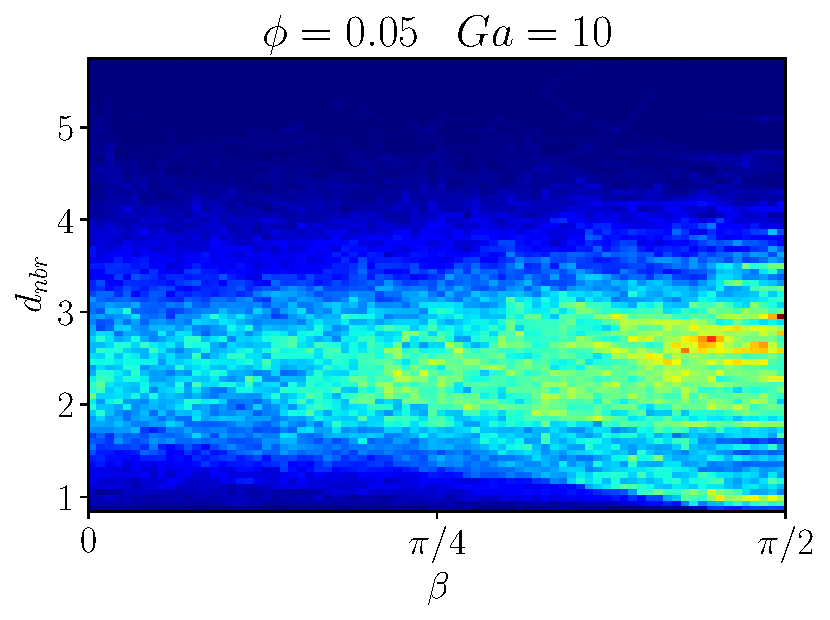
\includegraphics[width = 0.33\textwidth]{image/N_10/beta/2DMAP_beta_distmin_dmin_10_Bo1PHI0_05mu_r0_42Ga10.pdf}
    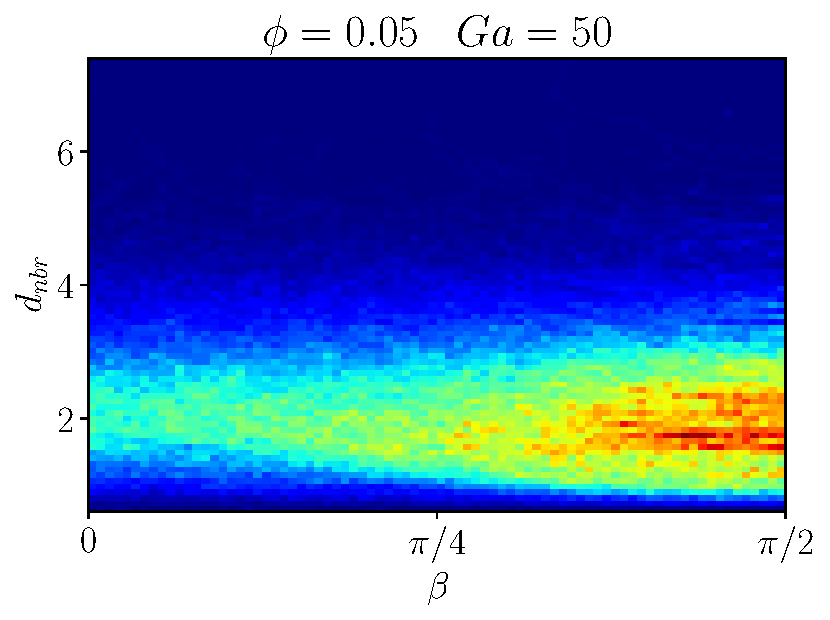
\includegraphics[width = 0.33\textwidth]{image/N_10/beta/2DMAP_beta_distmin_dmin_10_Bo1PHI0_05mu_r0_42Ga50.pdf}
    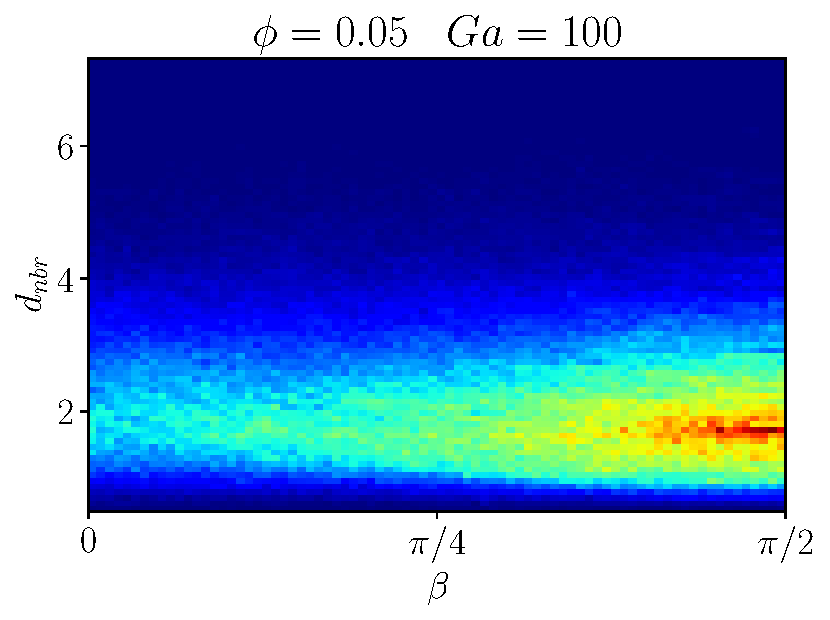
\includegraphics[width = 0.33\textwidth]{image/N_10/beta/2DMAP_beta_distmin_dmin_10_Bo1PHI0_05mu_r0_42Ga100.pdf}
    % 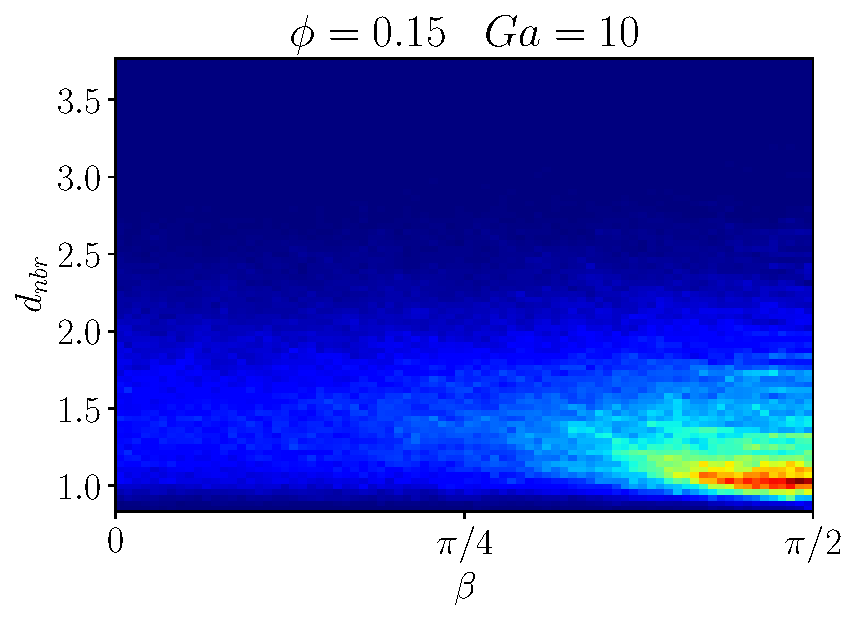
\includegraphics[width = 0.33\textwidth]{image/N_10/beta/2DMAP_beta_distmin_dmin_10_Bo1PHI0_15mu_r0_42Ga10.pdf}
    % 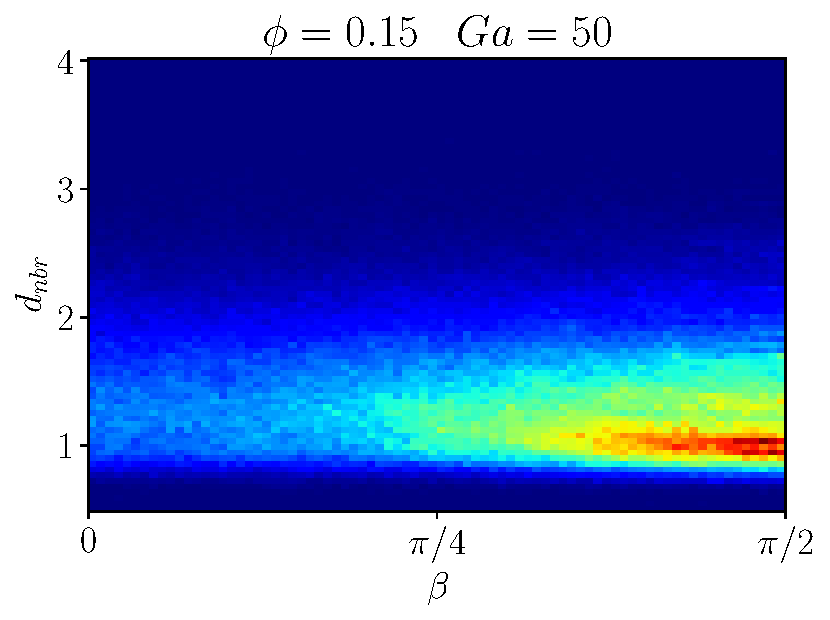
\includegraphics[width = 0.33\textwidth]{image/N_10/beta/2DMAP_beta_distmin_dmin_10_Bo1PHI0_15mu_r0_42Ga50.pdf}
    % 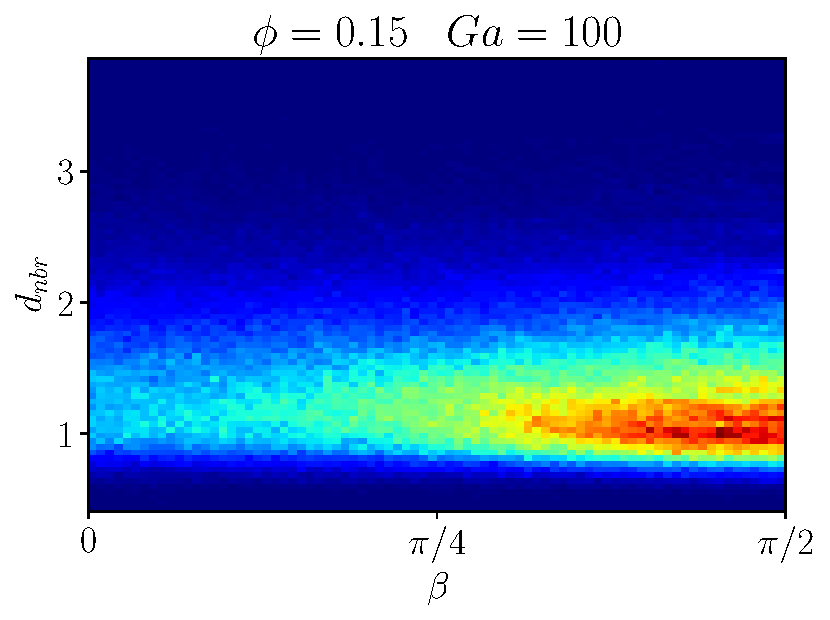
\includegraphics[width = 0.33\textwidth]{image/N_10/beta/2DMAP_beta_distmin_dmin_10_Bo1PHI0_15mu_r0_42Ga100.pdf}
    % 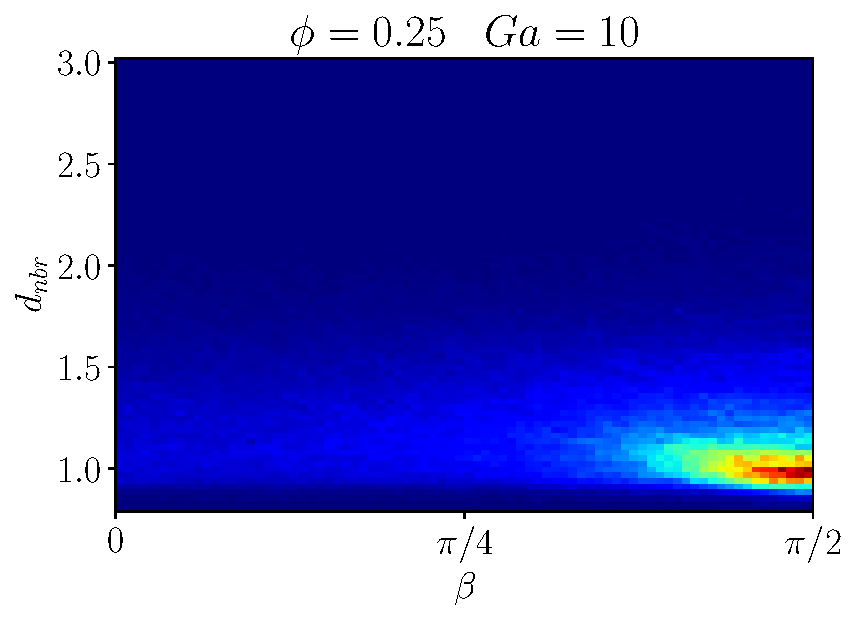
\includegraphics[width = 0.33\textwidth]{image/N_10/beta/2DMAP_beta_distmin_dmin_10_Bo1PHI0_25mu_r0_42Ga10.pdf}
    % 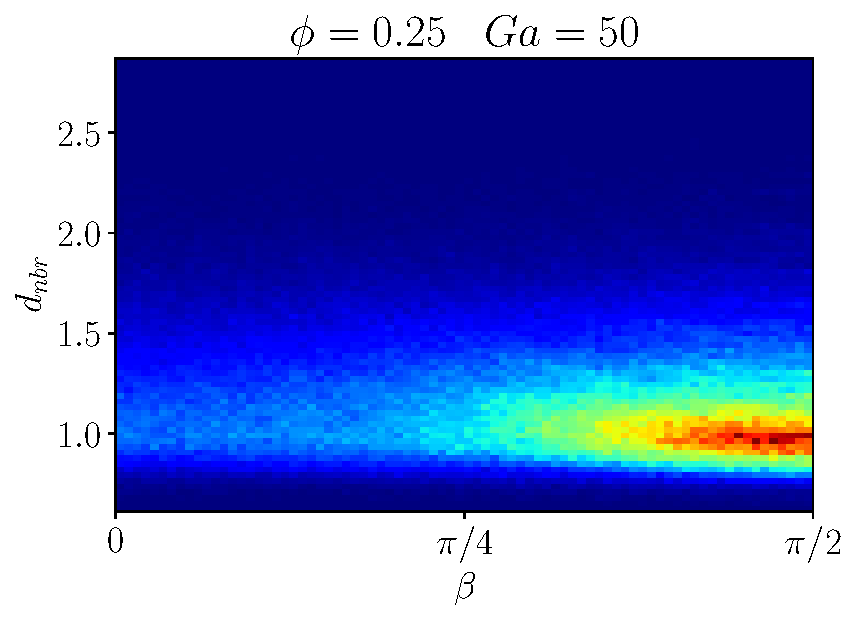
\includegraphics[width = 0.33\textwidth]{image/N_10/beta/2DMAP_beta_distmin_dmin_10_Bo1PHI0_25mu_r0_42Ga50.pdf}
    % 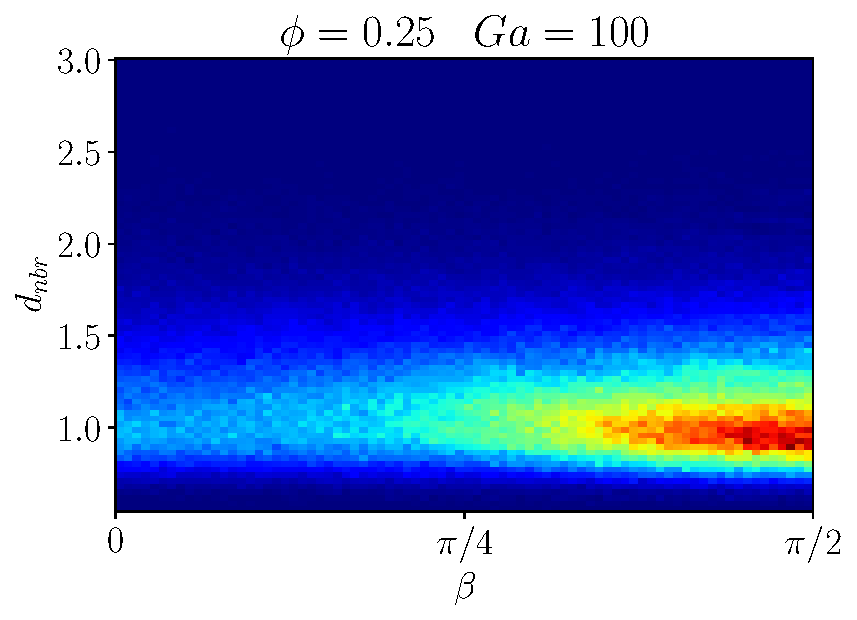
\includegraphics[width = 0.33\textwidth]{image/N_10/beta/2DMAP_beta_distmin_dmin_10_Bo1PHI0_25mu_r0_42Ga100.pdf}
    \caption{2 plots of $P_{\beta d_{nbr}}(\beta,d_{nrb})$ for different $\phi$ and $Ga$ at $Bo = 0.5$ and $\mu_r = 0.042$. The color represents the density, it goes from blue meaning $P_{\beta d_{nrb}}(\beta,d_{nrb})= 0$, to red meaning $P_{\beta d_{nrb}}(\beta,d_{nrb}) = P_{max}$. } 
\end{figure} 

$\triangleright$ As the particles get closer the contacts get more increasingly tangential. 

\end{frame}
\begin{frame}{2D density function of the angles distribution}
  \begin{figure}[h!]
    \centering
    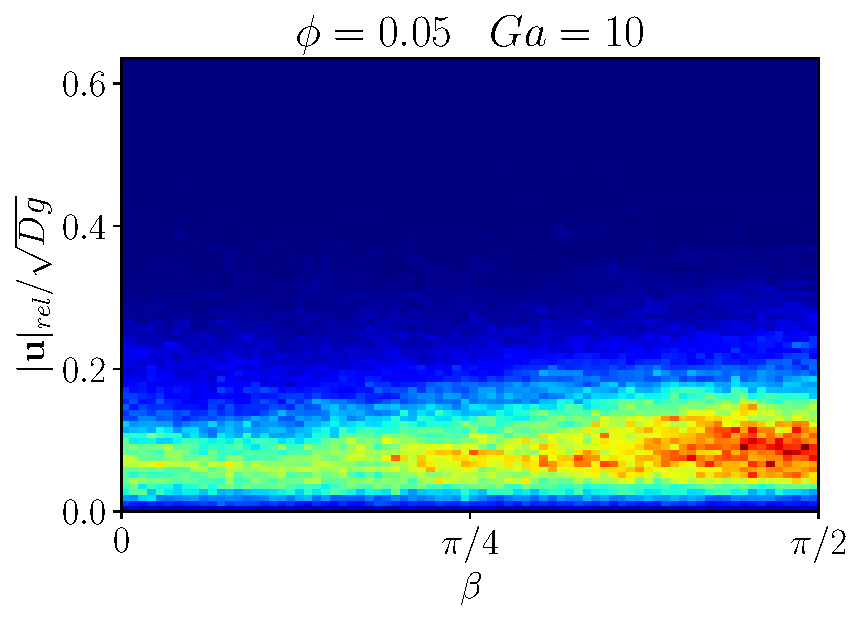
\includegraphics[width = 0.33\textwidth]{image/N_10/beta/2DMAP_beta_v_rel_dmin_10_Bo1PHI0_05mu_r0_42Ga10.pdf}
    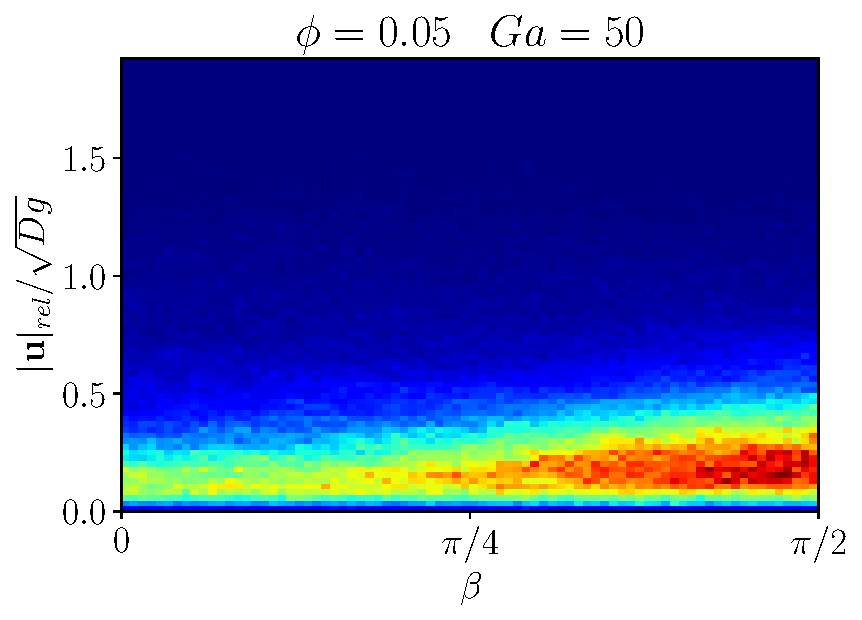
\includegraphics[width = 0.33\textwidth]{image/N_10/beta/2DMAP_beta_v_rel_dmin_10_Bo1PHI0_05mu_r0_42Ga50.pdf}
    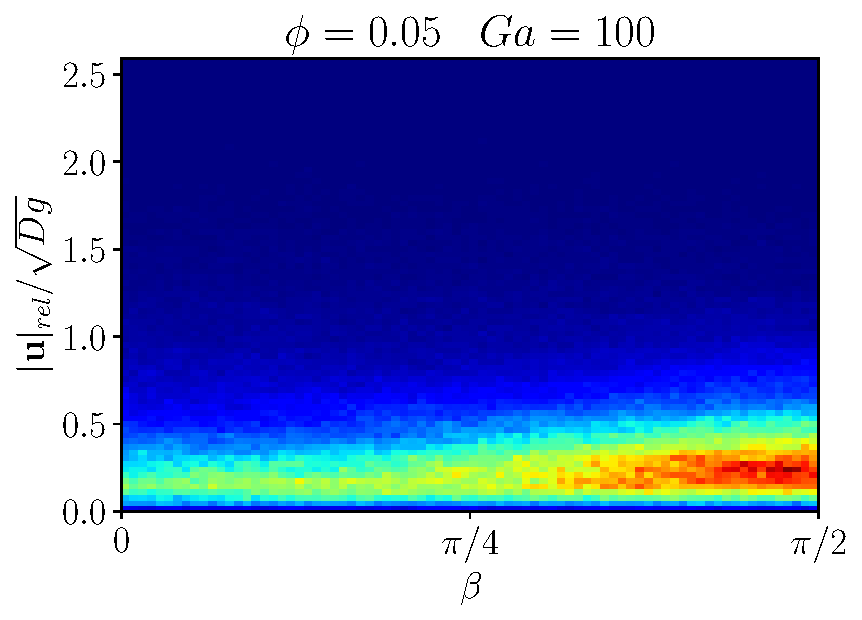
\includegraphics[width = 0.33\textwidth]{image/N_10/beta/2DMAP_beta_v_rel_dmin_10_Bo1PHI0_05mu_r0_42Ga100.pdf}
    % 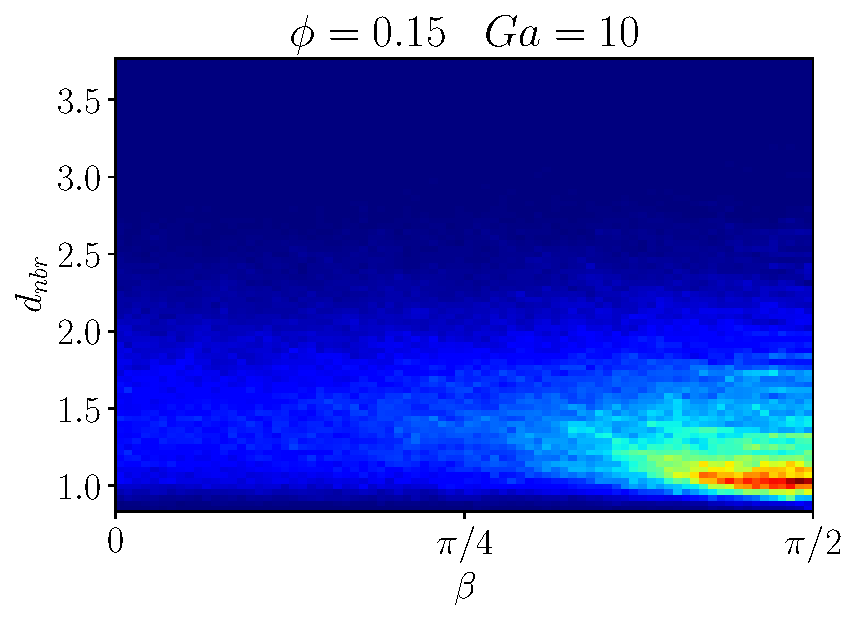
\includegraphics[width = 0.33\textwidth]{image/N_10/beta/2DMAP_beta_distmin_dmin_10_Bo1PHI0_15mu_r0_42Ga10.pdf}
    % 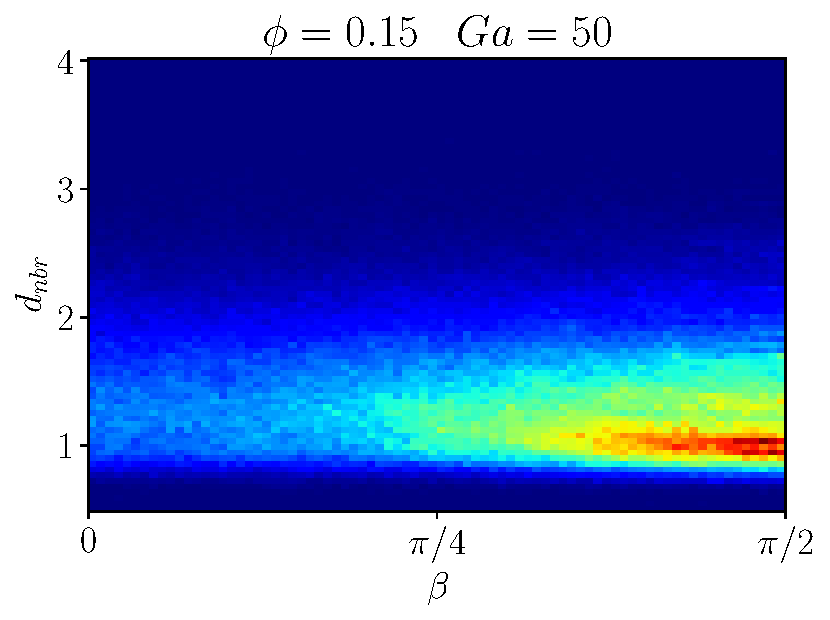
\includegraphics[width = 0.33\textwidth]{image/N_10/beta/2DMAP_beta_distmin_dmin_10_Bo1PHI0_15mu_r0_42Ga50.pdf}
    % 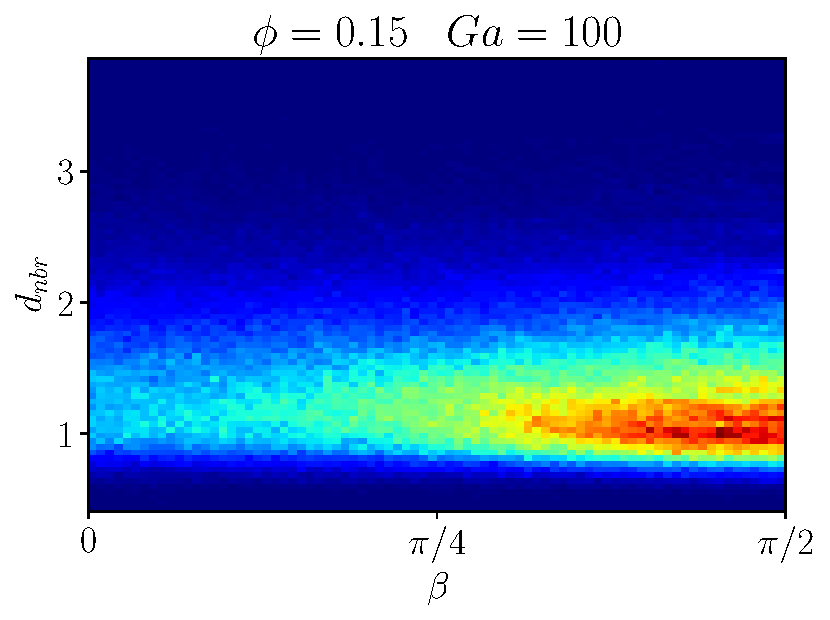
\includegraphics[width = 0.33\textwidth]{image/N_10/beta/2DMAP_beta_distmin_dmin_10_Bo1PHI0_15mu_r0_42Ga100.pdf}
    % 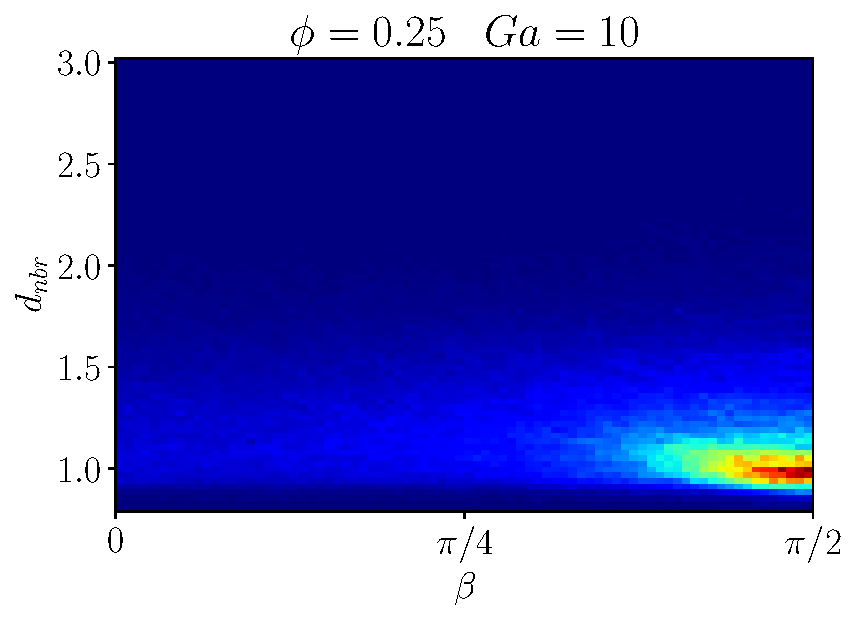
\includegraphics[width = 0.33\textwidth]{image/N_10/beta/2DMAP_beta_distmin_dmin_10_Bo1PHI0_25mu_r0_42Ga10.pdf}
    % 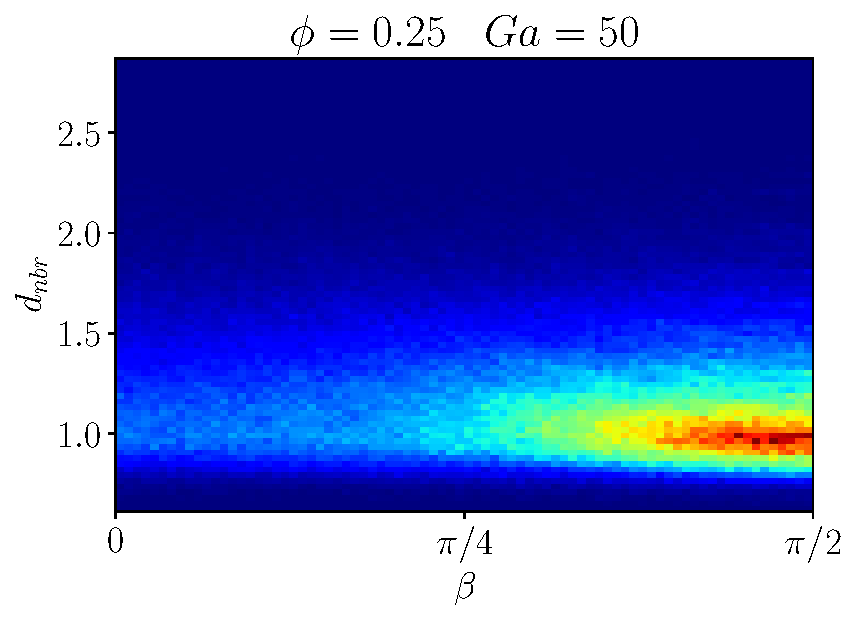
\includegraphics[width = 0.33\textwidth]{image/N_10/beta/2DMAP_beta_distmin_dmin_10_Bo1PHI0_25mu_r0_42Ga50.pdf}
    % 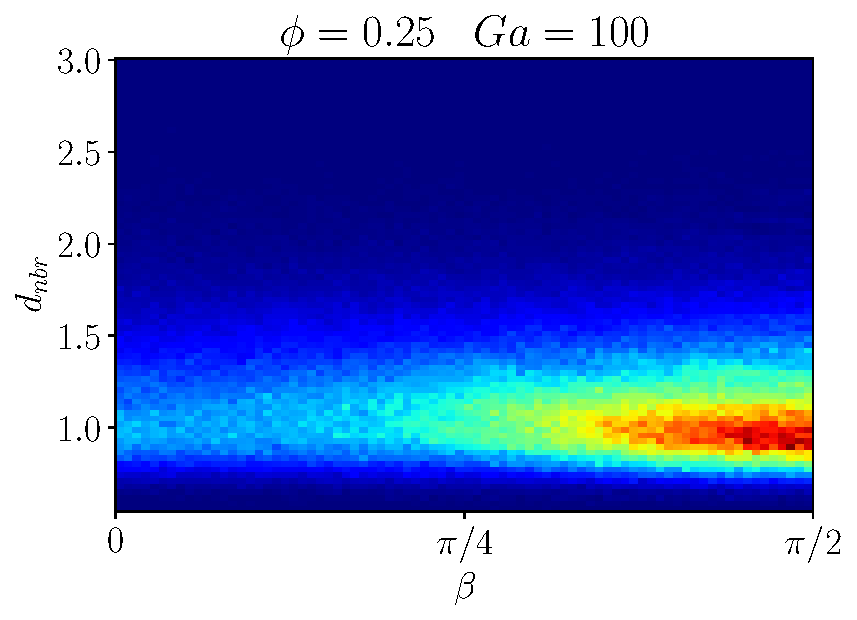
\includegraphics[width = 0.33\textwidth]{image/N_10/beta/2DMAP_beta_distmin_dmin_10_Bo1PHI0_25mu_r0_42Ga100.pdf}
    \caption{2 plots of $P_{\beta u_{rel}}(\beta,u_{rel})$ for different $\phi$ and $Ga$ at $Bo = 0.5$ and $\mu_r = 0.042$. The color represents the density, it goes from blue meaning $P_{\beta u_{rel}}(\beta,u_{rel})= 0$, to red meaning $P_{\beta u_{rel}}(\beta,u_{rel}) = P_{max}$.} 
\end{figure} 

% $\triangleright$ As the particles get closer the contacts get more increasingly tangential. 

\end{frame}

\begin{frame}{Bilan}
  \begin{columns}
    \begin{column}{0.7\textwidth}
      \begin{itemize}
        \item The droplets are in average close to each other of high $\phi$ and $Ga$. 
        \item The system is oriented horizontally at low $\phi$ 
        \item The interactions are tangential. 
        \item The interactions are even more tangential as the particles get closer. 
      \end{itemize}
    \end{column}
    \begin{column}{0.3\textwidth}
    \centering
    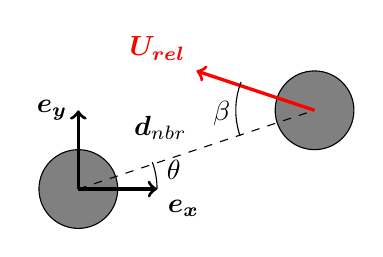
\begin{tikzpicture}
      \draw[fill=gray](0,0)circle (0.5);
      \draw[fill=gray](3,1)circle (0.5);
      \draw[dashed](0,0)--(3,1)node[midway,above left]{$\bm{d}_{nbr}$};
      \draw[very thick,->,red](3,1)--++(-1.5,0.5)node[above left]{$\bm{U_{rel}}$};
      \draw[very thick,->](0,0)--++(1,0)node[below right]{$\bm{e_x}$};
      \draw[very thick,->](0,0)--++(0,1)node[left]{$\bm{e_y}$};
      \draw(3,1)++(199:1)node[above left]{$\beta$} arc(199:159:1);
      \draw(0,0)++(0:1)node[above right]{$\theta$} arc(0:20:1);
    \end{tikzpicture} 
    \end{column}
  \end{columns}
\end{frame}


\section*{Additional results}
\begin{frame}{Time \& Frequency of the interactions}  
  \begin{figure}[h!]
    \centering
    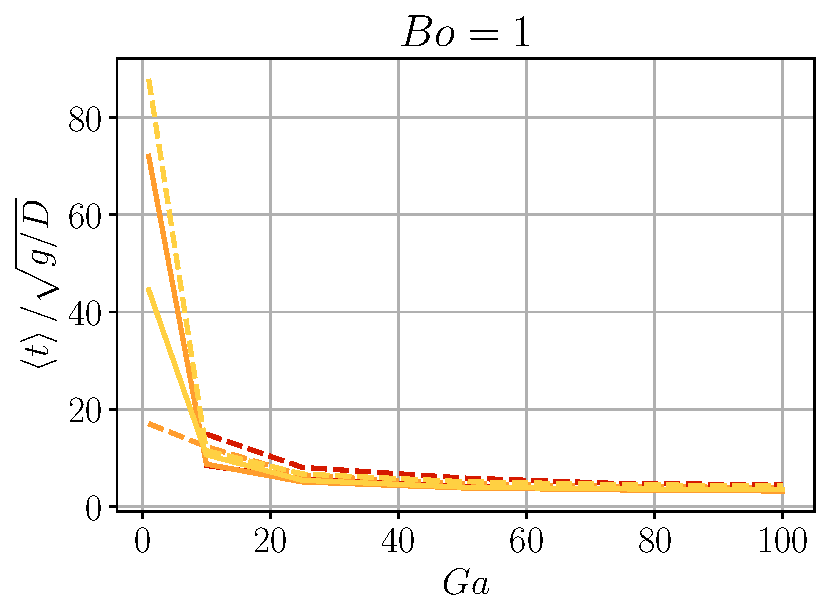
\includegraphics[width=0.33\textwidth]{image/N_10/time/Tcm_Bo_1.pdf}
    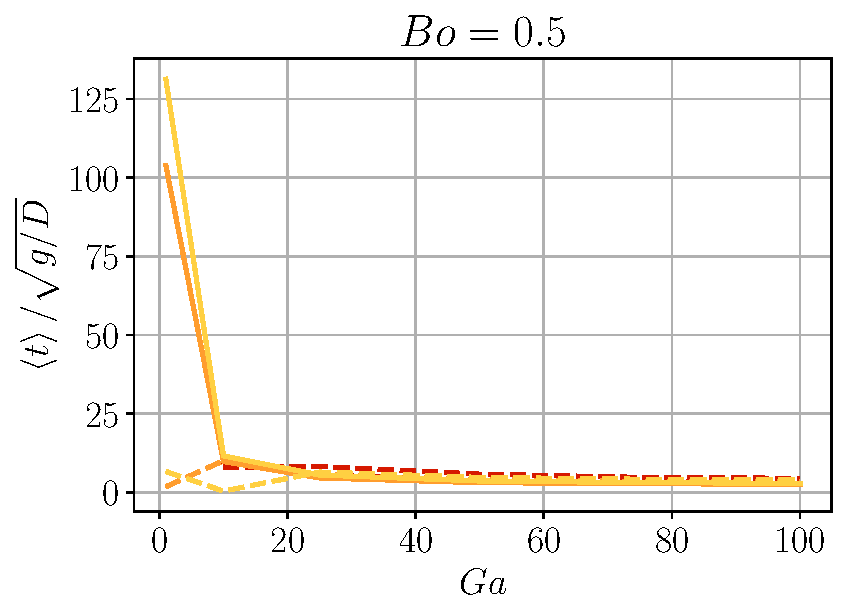
\includegraphics[width=0.33\textwidth]{image/N_10/time/Tcm_Bo_0_5.pdf}
    \caption{Averaged dimensionless time of contact. Dashed lines : $\mu_f = 0.42$, solid lines : $\mu_f = 0.042$. \textcolor{red}{\textbf{--}} : $\phi = 0.05$, \textcolor{orange}{\textbf{--}} : $\phi = 0.15$, \textcolor{yellow}{\textbf{--}} : $\phi = 0.25$} 
\end{figure} 
$\triangleright$ The contact time is inversely proportional to $Ga$. 
\end{frame}
\section*{Additional results}
\begin{frame}{Time \& Frequency of the interactions}  
  \begin{figure}[h!]
    \centering
    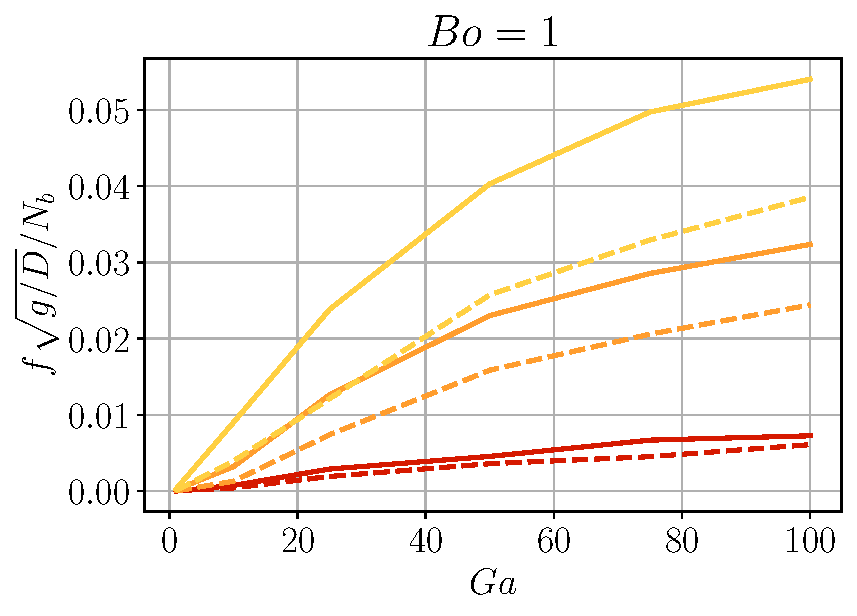
\includegraphics[width=0.33\textwidth]{image/N_10/freq/HzG_Bo_1.pdf}
    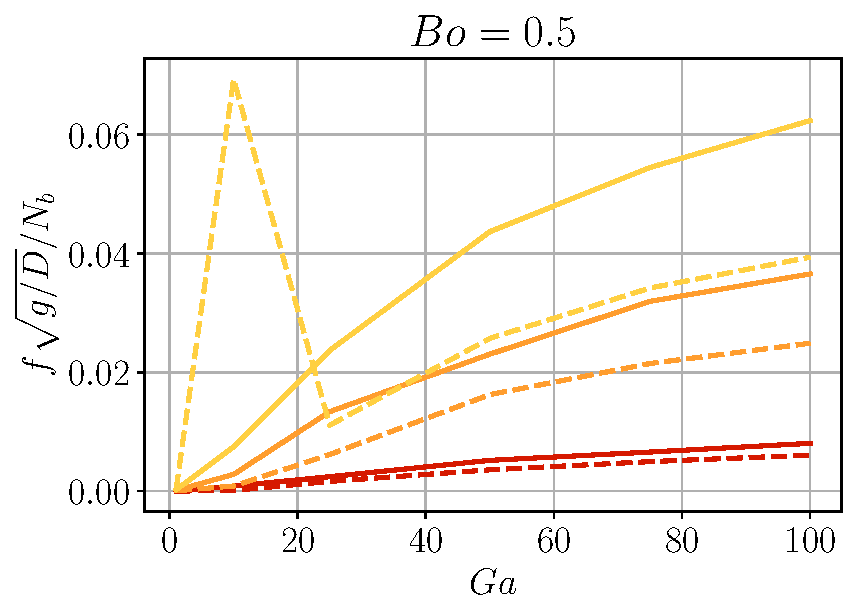
\includegraphics[width=0.33\textwidth]{image/N_10/freq/HzG_Bo_0_5.pdf}
    \caption{Dimensionless frequency of contact. Dashed lines : $\mu_f = 0.42$, solid lines : $\mu_f = 0.042$. \textcolor{red}{\textbf{--}} : $\phi = 0.05$, \textcolor{orange}{\textbf{--}} : $\phi = 0.15$, \textcolor{yellow}{\textbf{--}} : $\phi = 0.25$} 
\end{figure} 
\end{frame}

\backmatter

\end{document}
